\chapter{Introduction}

The Standard Model (SM) has been proven successful over the last decades by its accordance with results from many particle physics joint setups, the Super Proton Synchrotron (SPS)~\cite{Synchrotron:1997188} and its experiments created the experimental conditions to the discovery of the electroweak bosons, $W^{\pm}$ and $Z$. The Tevatron experiments (D0 , from Fermilab) allowed the discovery of the top quark. These were 3 of the four heaviest components of the SM. The missing piece was the, so called, Higgs Boson, or any other explanation to the mass of the other SM particles. 

In 2012, during CMS' Run1, at center-of-mass energy $\sqrt{s} = 7$ and $8$ TeV, researchers from CMS~\cite{Chatrchyan:2008zzk} and ATLAS~\cite{atlas_collaboration_2008}, two collaborations with experiments located at the Large Hadron Collider (LHC), a 27 km long circular proton-proton collider build and operated by CERN, announced the discovery a new particle~\cite{higgs_discovery_cms, higgs_discovery_atlas}, with characteristics compatibles with the Brout-Englert-Higgs boson, completing the SM picture proposed up to fifty years ago. In 2013, Francois Englert and Peter Higgs were awarded with the Noble Prize for \textit{"for the [...] discovery of a mechanism that contributes to our understanding of the origin of mass of subatomic particles, and which recently was confirmed through the discovery of the predicted fundamental particle, by the ATLAS and CMS experiments at CERN's Large Hadron Collider"~\cite{noble_prize}.}

On top of the success of the Higgs program at CMS, there is much to be understood, e.g. pin down the coupling constants of the Higgs boson with all three generations of quarks and leptons, its mass and its full width, evaluate non-zero CP-odd components in Higgs interactions, investigate double Higgs production and its self-coupling constant and possible extensions of the SM close to the Higgs sector and explore rare decays of Higgs. The former one, specially rare decays involving quarkonia, ,such as $H \rightarrow M \gamma$, where $M$ is a meson state, are a very good scenario to investigate the Higgs interaction with other SM particles other than the direct decay. This one would be overwhelmed by the immense background coming from QCD events. The same analogy can be extended to the Z boson, which also serves as a benchmark for the Higgs study.

The present study corresponds to 35.86 $fb^{-1}$ of data taken by CMS during 2016, during the Run2, at center-of-mass energy $\sqrt{s} = 13$ TeV, in which an upper limit on the branching fraction for $H/Z \rightarrow \Upsilon(1S, 2S, 3S) (\rightarrow \mu\mu) + \gamma $ is determined.

Because of its narrow resolution, muons play a special role not only for this study, but for CMS, in general. Not only the Higgs studies heavily depends of muonic final states (for decay channels, such as $H \rightarrow \mu\mu$ and $H \rightarrow ZZ \rightarrow 4l$ and identification of the production modes), but also muon final states are very important to a whole broad of physics process accessible at CMS/LHC. The Figure~\ref{dimuon_invariant_mass} presents the distribution of dimuon invariant mass reconstructed from different double muon triggers, with different requirements in pseudorapidity and transverse momentum. It is clear how the muons at CMS broaden the set of interesting process giving access to light quark hadrons to high transverse momentum phenomena.

% dimuon invariant mass
\begin{figure}[htbp]
    \centering
    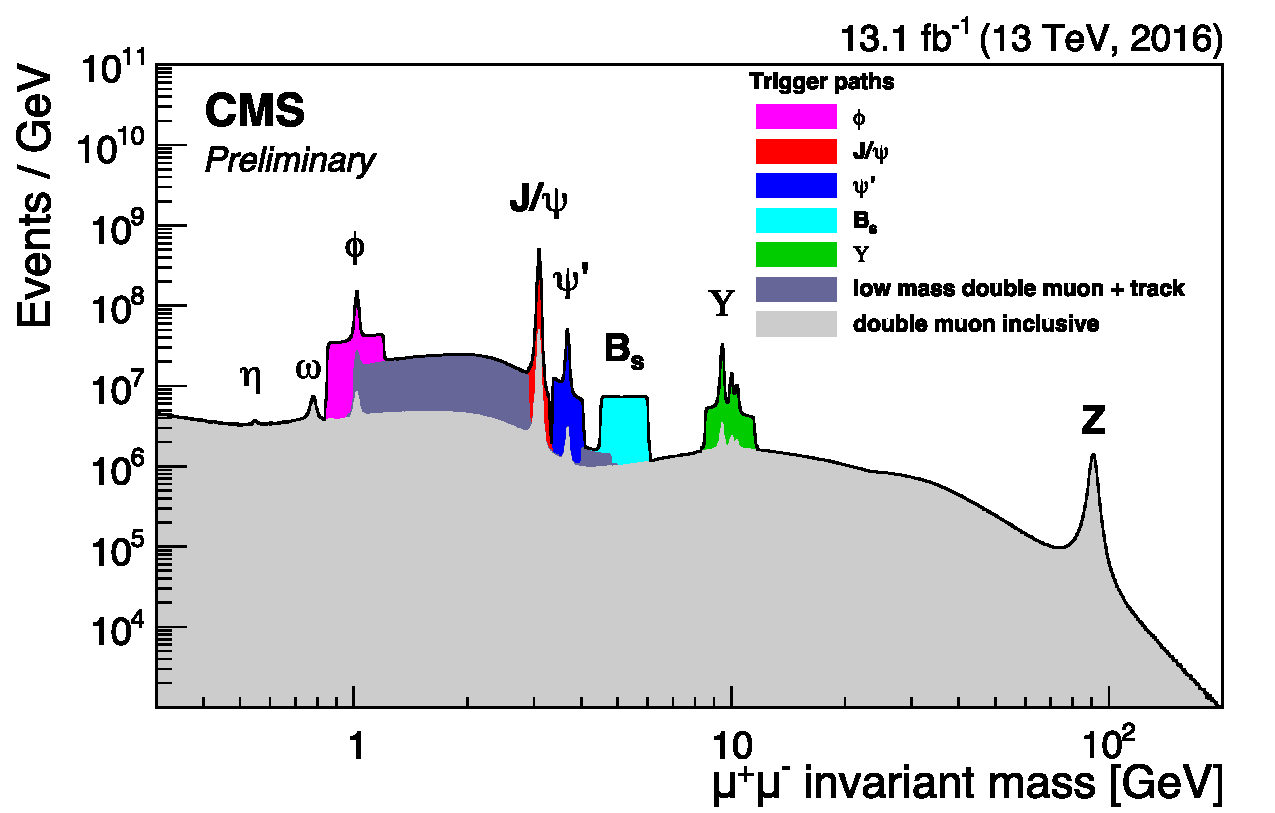
\includegraphics[width=0.7\textwidth]{figures_and_tables/introduction/dimuon_inv_mass.pdf}
    \caption{Dimuon mass distribution collected with various dimuon triggers. The light gray continuous distribution represents events collected with inclusive dimuon triggers with high $p_T$ thresholds. The dataset corresponding to an integrated luminosity of 13.1 $fb^{-1}$ was collected during the 25 ns LHC  running period at 13 TeV in 2016. Source:~\cite{dimuon_inv_mass}.}
    \label{dimuon_invariant_mass}
\end{figure}

In this scenario, a contribution to the muon system of CMS is a meaningful one to the collaboration. In this document we describe the contributions given to Resistive Plate Chamber (RPC) subdetector, including its commissioning, instrumentation for its upgrade, operation and maintenance.

This document is organized as follows: Chapter 1 is this introduction. Chapter 2 is devoted to a review of the theoretical foundations of this study and the motivations for the study of Rare Z and Higgs decays involving quarkonia. Chapter 3 is a review of the collider and experimental setup, LHC and CMS respectively. Chapter 4 is a review of the Resistive Plate Chamber technology for muon detection at CMS and the details of the contributions given to this subdetector. Chapter 5 is a detailed description of the data sample and the applied analysis procedure, as well as the statistical modeling and the branching fraction upper limit extraction. Chapter 6 presents a summary and perspectives for future developments.

Wherever figures and tables sources are not provided, the source is the author himself.

In this document, the convention of natural units is implicitly used: the vacuum speed of light ($c$), the reduced Planck constant ($\hbar$) and electric permittivity ($\epsilon_{0}$) are normalized to unity. In this way, SI units are:
\begin{itemize}
    \setlength\itemsep{-0.5em}
    \item mass ($[m]$) = GeV,
    \item energy ($[E]$) = GeV,
    \item momentum ($[p]$) = GeV,
    \item time ($[t]$) = 1/GeV,
    \item length ($[s]$) = 1/GeV.
\end{itemize}

The summation convention is also followed. In this notation, $y = A^i B_i$ stands for $y = \sum_{i=0}^n A^i B_i = A^1 B_1 + A^2 B_2 + A^3 B_3 + ... + A^n B_n$.